\section[约束秩亏问题]{约束秩亏问题\\Constraining a rank Deficient Problem}	
\par \noindent
当$A$列相关时,奇异最小二乘问题有无数个解(与$Ax= \mathbf{0}$不同):
\begin{center}
	选择最佳估值 $\hat{x}$使得$||{x - Ax}||$最小。
\end{center}
我们通过增加如下$d$个附加约束条件寻找唯一解
\begin{equation}
	G^\mathsf{T}x
	=g\text{。}
\end{equation}
这里$d = n - r$ 等于$A$的列数减去 $A$ 互相独立的列数(即矩阵 $A$ 的秩)。由矩阵$G$的$d$个新列增强的矩阵$A$是满秩的并且秩为$n$。
\par
我们将这个问题当做由奇异矩阵$A^\mathsf{T}A$组成的问题,并且通过\emph{正交加边化矩阵}$G$将它公式化:
\begin{equation}
	\begin{bmatrix}
		A^\mathsf{T}A & G \\
		G^\mathsf{T} & \mathbf{0}
	\end{bmatrix}
	\begin{bmatrix}
		x\\
		\mathbf{0}
	\end{bmatrix}
	=
	\begin{bmatrix}
		A^\mathsf{T}b \\ g
	\end{bmatrix}\text{。}
\end{equation}
通过矩阵$G^\mathsf{T}$对$A^\mathsf{T}A$的增强使分块矩阵可逆。这时的解是唯一的,而且它可以用广义逆 $A^\mathsf{+}$的形式表示:
\begin{equation}
	x^\mathsf{+}
	=A^\mathsf{+}b\text{。}
\end{equation}
\textbf{备注 7.2} 这个问题有另外一种公式化形式。法方程为
\begin{equation}
	A^\mathsf{T}Ax
	=A^\mathsf{T}b\text{。}
\end{equation}
$A^\mathsf{T}A$仍然是奇异的和非负的。为了获得唯一解,我们增加了一个合适的\emph{虚拟观测方程}
\begin{equation}
	Fx
	=g\text{。}
\end{equation}
现在我们考虑矩阵
$\begin{bmatrix}
A\\
F
\end{bmatrix}$
的未加权的最小二乘问题,该矩阵为列满秩矩阵。假设这些观测方程是权重归一化的,法方程就变为:
\begin{equation}
	(A^\mathsf{T}A + F^\mathsf{T}F)x
	=A^\mathsf{T}b + F^\mathsf{T}g \text{。}
\end{equation}
这样一种对问题的补充称为\emph{软公设}。我们将会看到这个软公设如何决定系数矩阵的逆。
\par
如果给予虚拟观测值无限权重—\emph{硬公设},这意味着式(7.18)被强制执行—那么这些方程被视为条件方程而不是观测方程。
\par
我们展示下面式(7.44)的转换过程。并且将它的软假设进行如下修改:
\begin{equation}
	\sum\nolimits_ {\text{transformed}}
	=S(\sum\nolimits_{\hat{x}} + G^\mathsf{T})S^\mathsf{T}\text{。}
\end{equation}
根据Krarup(1979)所知。
\par\noindent
\textbf{例 7.2} 定向图如图7.2所示,图中给出了各边的高度差。与这张图相关的关联矩阵是
\begin{equation*}
	A
	=
	\begin{bmatrix}
		-1 & 0 & 0 & 1 & 0\\
		-1 & 0 & 0 & 0 & 1\\
		0 & 0 &-1 & 1 & 0\\
		0 &-1 & 0 & 0 & 1\\
		0 & 0 & 0 & 1 & -1
	\end{bmatrix}
\end{equation*}
其中观测值是
\begin{equation*}
	b
	=
	\begin{bmatrix}
		1.978\\
		0.732\\
		0.988\\
		0.420\\
		1.258
	\end{bmatrix}\text{。}
\end{equation*}
\begin{figure}
	\centering
	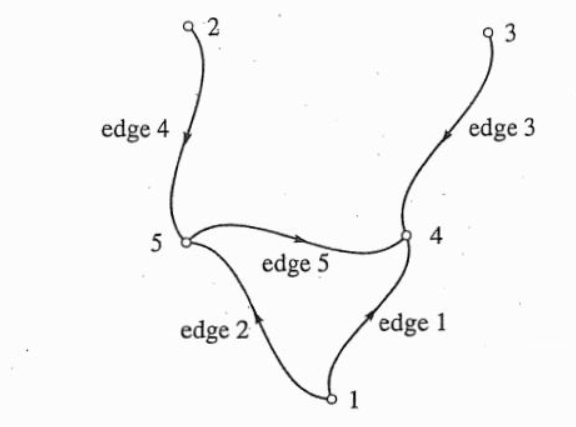
\includegraphics[width=0.4\linewidth]{TeX_files/Part02/chapter07/image/7-2}
	\caption{图7.2 定向自由水准网图}
	\label{fig:7-2}
\end{figure}

\par\noindent
矩阵$A^\mathsf{T}A$ 是奇异的。$A$的唯一解可以通过广义逆矩阵 $A^\mathsf{+}$计算出。这个矩阵通过$A$的奇异分解确定。此分解为$A = U\sum V^\mathsf{T}$,在7.1节已解释了广义逆:$A^+ 
= V\sum^{+}U^\mathsf{T}$。最小范数的唯一最小二乘解是
\begin{equation*}
	x^+
	= A^{+}b
	=
	\begin{bmatrix}
		-0.8024\\
		-0.4944\\
		0.1916\\
		1.1796\\
		-0.0744
	\end{bmatrix}\text{。}
\end{equation*}
通过用行矩阵$e^\mathsf{T}$增强矩阵$A^\mathsf{T}A$与所有的列向量$e$得到$\hat{x} = x^{+}$,列向量$e$来自$A$的零空间:
\begin{equation*}
	\begin{bmatrix}
		A^\mathsf{T}A & e \\
		e^\mathsf{T} & \mathbf{0}
	\end{bmatrix}
	\begin{bmatrix}
		x\\
		\mathbf{0}
	\end{bmatrix}
	=
	\begin{bmatrix}
		A^\mathsf{T}b \\
		\mathbf{0}
	\end{bmatrix}\text{。}
\end{equation*}
请注意,均值$\hat{x} = \hat{x}_{0}$=0。这个给出了最后的方程$e^\mathsf{T}\hat{x} = \mathbf{0}$。为了求得解,我们没有使用法方程而是使用奇异值分解。
\par
如果我们想要从“0级”到一级改变解$\hat{x}_{0}$比如$l$ = 20。我们只需要将$g$变为5 $\times$ 20 = 100,我们得到解
\begin{equation*}
	\hat{x}_{20}
	=     \begin{bmatrix}
		19.1976\\
		19.5056\\
		20.1916\\
		21.1796\\
		19.9256
	\end{bmatrix}\text{。}
\end{equation*}
因为$e^\mathsf{T}\hat{x}_{20} = 100$,所以这个解的平均值是20。
\par\noindent
\textbf{例7.3} 我们想要证明一个投影如何从将例7.2的$\hat{x}_{20}$带回到$\hat{x}_{0}$。在这种特殊情况下,我们投影到与$e$垂直的平面。这个投影矩阵是
\begin{equation*}
	P
	= I - e(e^\mathsf{T}e)^{-1}e^\mathsf{T}
	= I - \frac{1}{5}ee^\mathsf{T}
	= \frac{1}{5}
	\begin{bmatrix}
		4 & -1 & -1 & -1 & -1\\
		-1 & 4  & -1 & -1 & -1\\
		-1 & -1 &  4 & -1 & -1\\
		-1 & -1 & -1 &  4 & -1\\
		-1 & -1 & -1 & -1 & 4\\
	\end{bmatrix}
\end{equation*}
或者
\begin{equation*}
	\hat{x}_{0}
	=P\hat{x}_{20}
	= p
	\begin{bmatrix}
		19.1976\\
		19.5056\\
		20.1916\\
		21.1796\\
		19.9256
	\end{bmatrix}
	=\begin{bmatrix}
		-0.8024\\
		-0.4944\\
		0.1916\\
		1.1796\\
		-0.0744
	\end{bmatrix}\text{。}
\end{equation*}
\textbf{例7.4} 继续例7.2,我们将计算出伪逆解的协方差阵。我们将确定标准差(单位权的标准差)$b - Ax^{+} = b - AA^{+}b = (I - AA^{+})b$ 和 $\hat{\sigma}_0 = ||b - Ax^{+}|| = 
0.0069 = 6.9mm$。
\par\noindent
因此协方差矩阵$\Sigma_+ = {\hat{\sigma}_0}^2\emph{A}^{+}(\emph{A}^{+})^\mathsf{T}$ 是
\begin{equation*}
	\begin{bmatrix}
		0.192 & -0.096 & -0.096 & -0.000 & -0.000\\
		-0.096 & 0.416  & -0.224 & -0.128 & 0.032\\
		-0.096 & -0.224 & 0.416  & 0.032  & -0.128\\
		-0.000 & -0.128 & 0.032  & 0.128  & -0.032\\
		-0.000 & 0.032  & -0.128 & -0.032 & 0.128\\
	\end{bmatrix}\times10^{-4}\text{。}
\end{equation*}
其中迹线$(\sum_+) = 1.280 \times 10^{-4}$。接下来,我们得到
\begin{equation*}
	Bx
	=
	\begin{bmatrix}
		A\\
		e^\mathsf{T}
	\end{bmatrix}
	x
	=
	\begin{bmatrix}
		b\\
		\mathbf{0}
	\end{bmatrix}
\end{equation*}
并且$\sum = {\hat{\sigma}_0}^2(B^\mathsf{T}B)^{-1}$变为
\begin{equation*}
	\begin{bmatrix}
		0.211 &-0.077 &-0.077 &0.019  &0.019\\
		-0.077 &0.435  &-0.205 &-0.109 &0.051\\
		-0.077 &-0.205 &0.435  &0.051  &-0.109\\
		0.019 &-0.109 &0.051  &0.147  &-0.013\\
		0.019  &0.051  &-0.109 &-0.013 &0.147\\
	\end{bmatrix}\times10^{-4}\text{。}
\end{equation*}
最终迹线$(\sum) = 1.376 \times 10^{-4}$。很明显迹线$(\sum_+)$$ <$迹线$(\sum)$。
\par\noindent
\textbf{例7.5} 这是一个\emph{自由网}的例子,为了包含网中其他点的未知数我们增加$n = 2$个原始未知数。因此未知数的数量增加到8。因为$A$的秩等于$8 - 3 = 5$,we have to include at 
least
\begin{figure}
	\centering
	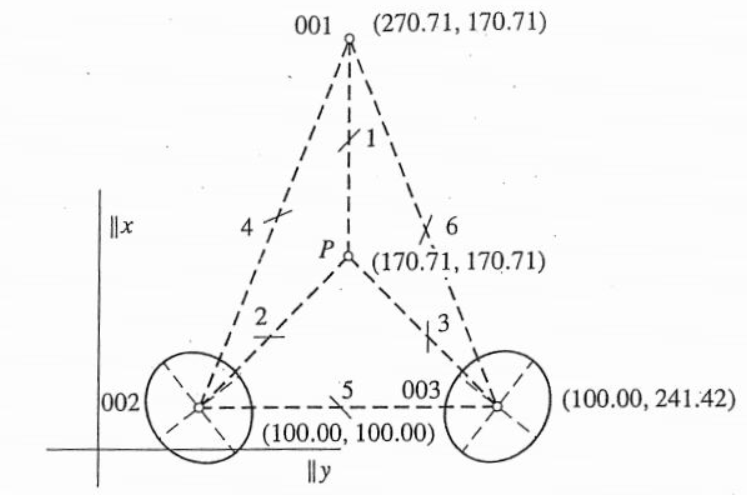
\includegraphics[width=0.4\linewidth]{TeX_files/Part02/chapter07/image/7-3}
	\caption{}
	\label{fig:7-3}
\end{figure}
\par\noindent
\textbf{图7.3} 自由距离网有6个观测值。置信椭圆与假定坐标$X_P$,$Y_P$,$X_{001}$,与 $Y_{001}$相对应。
\par\noindent
与例7.1相比这里有更多的观察值。由于对称,我们甚至推断出多余三个的观测值即距离观测值在001与002之间 ,002与003之间,003与001之间。未知数向量是
\begin{equation*}
	x =
	\begin{pmatrix}
		x_P,y_P,x_{001},y_{001},x_{002},
		y_{002},x_{003},y_{003}
	\end{pmatrix}\text{。}
\end{equation*}
这个增强系数矩阵是6行8列,秩为4:
\begin{equation*}
	A =
	\begin{bmatrix}
		-1 & 0 & 1 & 0 & 0 & 0 & 0 & 0\\
		0.707 & 0.707 & 0 & 0 & -0.707 & -0.707 & 0 & 0\\
		0.707 &-0.707& 0 &0 &0& 0& -0.707& 0.707\\
		0 & 0 &0.924& 0.383& -0.924 &-0.383& 0& 0\\
		0& 0 &0 &0 &0 &-1& 0& 1\\
		0& 0 &0.924 &-0.383& 0& 0&\ -0.924& 0.383
	\end{bmatrix}\text{。}
\end{equation*}
我们在$G^\mathsf{T}$的行中为4维度的零空间选择了一个基础:
\begin{equation*}
	G^\mathsf{T} =
	\begin{bmatrix}
		1 & 0 & 1 & 0 & 1 & 0 & 1 & 0\\
		0 & 1 & 0 & 1 & 0 & 1 & 0 & 1\\
		-170.71 & 170.71 &-170.71& 270.71& -100 &100& -241.42& 100\\
		\quad170.71& 170.71 &\quad270.71 &170.71& \quad100& 100& 100& \quad241.42
	\end{bmatrix}
\end{equation*}
并且右边是
\begin{equation*}
	b
	=\begin{bmatrix}
		0.010\\
		0.020\\
		0.030\\
		0.010\\
		0.020\\
		0.030
	\end{bmatrix}\text{。}
\end{equation*}
伪逆解$x^+ = A^+b$并且残差$b - Ax^+$是
\begin{equation*}
	b
	=\begin{bmatrix}
		\quad 0.008 0\\
		\quad0.002 3\\
		\quad0.0113\\
		-0.0068\\
		-0.0026\\
		-0.0087\\
		-0.0167\\
		0.013 2
	\end{bmatrix}
	\qquad \text{和}  \qquad
	b- Ax^+
	=\begin{bmatrix}
		\quad0.0067\\
		\quad0.0047\\
		\quad0.0047\\
		-0.0036\\
		-0.0020\\
		-0.0036
	\end{bmatrix}\text{。}
\end{equation*}
标准差$\hat{\sigma_0} = 10.9mm$。自由网的最小二乘解取决于以下坐标$(X_{i}^{'},Y_{i}^{'})$:
\par
\begin{tabular}{ccccccc}
	Point & $X_i$ & $\xi_i$ & $X_{i}^{'}$ & $Y_i$ & $\eta_i$ & $Y_{i}^{'}$\\
	\hline
	P & 170.71 & 0.008 & 170.718 & 170.71 &\quad 0.002 &170.71\\
	1 &270.71  & 0.011 &270.721  &170.71  &-0.007 &170.703\\
	2 &100.00  &-0.003 &99.997   &100.00  &-0.009 &99.991\\
	3 &100.00  &-0.017 &99.983   &241.42  &\quad0.013  &241.433
\end{tabular}
\par\noindent
注意在计算精度之内$\sum{\xi_{i}} = \sum_{\eta_i} = 0$。
